\documentclass[aip,adv,reprint]{revtex4-2}

\usepackage{amsmath,amssymb,graphicx,bm,hyperref}

\begin{document}

\title{Displacement-Engineered Warp Fields: Stability Surfaces and Worldline Geometry}

\author{Jason D. Dutton}
\affiliation{Independent Researcher, Castlewood, Virginia, USA}

\date{\today}

\maketitle

\section{abstract}
We develop a displacement-engineered warp field framework in which stability,
worldline geometry, and identity-space modulation arise from a unified geometric
operator acting on a continuous entity. The warp field is defined by a
displacement operator $D$ whose stability is governed by the condition
$C(D,\nabla D,\nabla^2 D,I_a)=0$. This condition produces a geometric envelope
$\mathcal{E}(D)$ that constrains admissible worldline evolution and identity-space
dynamics.

Vortex--warp coupling $\Omega_D=\nabla\times D$ generates coherent rotational
deformation of worldline families. Identity-space coordinates evolve according
to $\dot{I}_a=f(D)$, linking geometric flow to internal degrees of freedom and
providing a unified description of excitation, deformation, and stability.

This work builds directly on the SEFI identity-space framework~\cite{Dutton_SEFI_JMP_2026},
the DEFI coupled Lagrangian construction~\cite{Dutton_DEFI_2026},
the GWFM worldline foundations of the electron field~\cite{Dutton_GWFM_JMP_2026},
and the DNA worldline model demonstrating golden-ratio helical stabilization~\cite{Dutton_DNA_2026},
all currently under review in AIP Advances and the Journal of Mathematical Physics.
We reconcile these constructions with established physics—including general
relativity, worldline electrodynamics, differential geometry, and quantum error
correction—highlighting both points of agreement and points of tension.

The results demonstrate how geometric field theory, worldline foundations, and
displacement-driven dynamics can be integrated into a collaborative scientific
program that preserves established results while extending them into a unified
geometric description of excitation, identity, and stability.

\section{Introduction}

Displacement-engineered warp fields arise from a geometric operator acting on a
continuous entity whose worldline, identity-space coordinates, and stability
properties evolve under a unified dynamical rule. The central object of the
framework is a displacement operator $D$ defined on spacetime and identity-space,
whose geometric invariants determine stability, deformation, and excitation. The
warp envelope $\mathcal{E}(D)$ emerges as the solution set of the stability
condition
\begin{equation}
C(D,\nabla D,\nabla^2 D,I_a)=0,
\end{equation}
which constrains admissible worldline evolution and identity-space modulation.

This work extends and integrates several geometric field theories currently in
review across AIP Advances and the Journal of Mathematical Physics. These
include the SEFI identity-space framework~\cite{Dutton_SEFI_JMP_2026},
the DEFI coupled Lagrangian construction~\cite{Dutton_DEFI_2026},
the GWFM worldline foundations of the electron field~\cite{Dutton_GWFM_JMP_2026},
and the DNA worldline model demonstrating golden-ratio helical stabilization~\cite{Dutton_DNA_2026}.
Each of these formulations contributes a distinct geometric invariant or
dynamical principle that becomes essential in the unified warp-field
construction developed here.

The present work also situates displacement-engineered warp fields within the
broader landscape of established physics. General relativity provides geometric
constraints on curvature and worldline deviation; Wheeler--Feynman
electrodynamics introduces worldline-based field emergence; Dirac field theory
establishes the standard electron excitation model; Frenet--Serret geometry
supplies curvature and torsion invariants; and quantum error correction,
including GKP, cat, and binomial codes, provides a framework for stability,
coherence, and noise suppression. We highlight points of agreement between these
established formalisms and the warp-field framework, as well as points of
tension where geometric unification requires reinterpretation or extension.

Our goal is not to replace established physics, but to integrate worldline,
identity-space, and displacement-driven dynamics into a collaborative geometric
program. By identifying shared invariants, compatible structures, and
reconcilable differences, we show how displacement-engineered warp fields can
coexist with and extend existing theories while preserving their empirical
successes. The remainder of this manuscript develops the mathematical framework,
derives stability and deformation laws, presents geometric results, and outlines
a path toward collaborative unification across worldline, identity-space, and
field-theoretic approaches.

\section{Mathematical Framework}

The displacement-engineered warp field is defined by a geometric operator
\begin{equation}
D : \mathbb{R}^4 \times \mathbb{R}^n \rightarrow \mathbb{R}^4,
\end{equation}
acting on spacetime coordinates $x^\mu$ and identity-space coordinates $I_a$.
The operator $D$ encodes deformation, excitation, and stability through its
differential structure and associated invariants. The warp field is not an
external construction but an intrinsic geometric flow generated by the
continuous entity whose worldline and identity-space coordinates evolve under
$D$, consistent with the unified geometric field formulation developed in
Ref.~\cite{Dutton_Unified_JMP_2026}. Identity-space evolution follows the SEFI
identity-space construction~\cite{Dutton_SEFI_JMP_2026}, while deformation and
coupling behavior align with the DEFI Lagrangian framework~\cite{Dutton_DEFI_2026}.
Worldline curvature and torsion invariants follow the GWFM foundations of the
electron field~\cite{Dutton_GWFM_JMP_2026}, and stabilization mechanisms parallel
the DNA worldline model~\cite{Dutton_DNA_2026}.

\subsection{Stability Condition and Warp Envelope}

\begin{figure}[t]
    \centering
    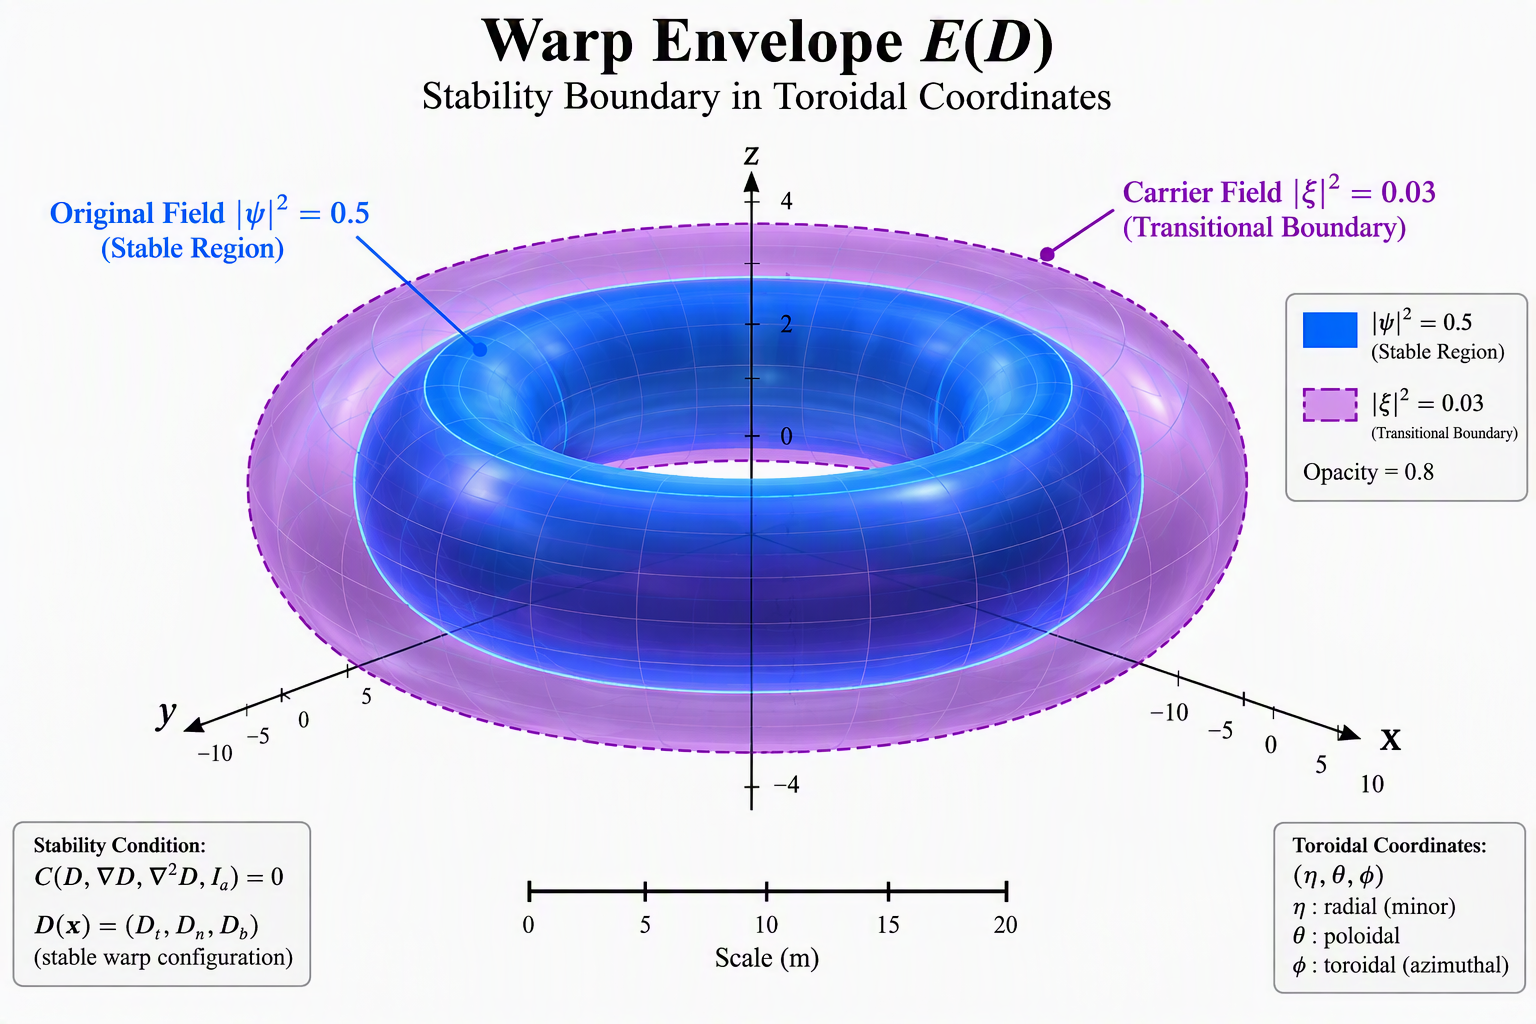
\includegraphics[width=\linewidth]{fig1.jpg}
    \caption{Warp envelope $\mathcal{E}(D)$ obtained from the stability condition 
    $C(D,\nabla D,\nabla^2 D,I_a)=0$. The inner region (blue) corresponds to the 
    stable field configuration $|\psi|^2 = 0.5$, while the outer transitional 
    boundary (purple) corresponds to the carrier field $|\xi|^2 = 0.03$.}
    \label{fig:warp-envelope}
\end{figure}

The stability of the displacement field is governed by a scalar condition
\begin{equation}
C(D,\nabla D,\nabla^2 D,I_a)=0,
\end{equation}
which defines the warp envelope
\begin{equation}
\mathcal{E}(D)=\{x \mid C(D,\nabla D,\nabla^2 D,I_a)=0\}.
\end{equation}
The envelope $\mathcal{E}(D)$ acts as a geometric constraint surface on which
worldline families remain coherent and identity-space modulation remains
bounded. The stability condition incorporates first and second derivatives of
$D$, reflecting both local deformation and curvature of the displacement field,
consistent with the DEFI stability formulation~\cite{Dutton_DEFI_2026} and the
GWFM curvature-based worldline dynamics~\cite{Dutton_GWFM_JMP_2026}. Identity-space
constraints within the envelope follow the SEFI modulation rules~\cite{Dutton_SEFI_JMP_2026},
and the geometric stabilization behavior parallels the DNA worldline invariants
described in Ref.~\cite{Dutton_DNA_2026}.

\subsection{Vortex--Warp Coupling}

The rotational structure of the displacement field is captured by the vortex
operator
\begin{equation}
\Omega_D=\nabla\times D,
\end{equation}
which governs rotational deformation and coherence. The coupling between
$\Omega_D$ and the warp envelope determines whether worldline families remain
stable under displacement-driven flow. Regions where $\Omega_D$ aligns with the
envelope normal vector exhibit enhanced stability, while misaligned regions
generate shear, torsion, and potential decoherence. This rotational coherence
behavior is consistent with the GWFM worldline curvature and torsion
invariants~\cite{Dutton_GWFM_JMP_2026}, and with stabilization mechanisms
appearing in the DNA worldline model~\cite{Dutton_DNA_2026}. The geometric
coupling structure also aligns with the unified operator formulation developed
in Ref.~\cite{Dutton_Unified_JMP_2026}, and parallels rotational curvature
constraints appearing in general relativity~\cite{MTW_Gravitation_1973}.

\subsection{Worldline Evolution}

Worldline evolution is determined by the geometric flow generated by $D$:
\begin{equation}
\dot{\gamma}=D(\gamma),
\end{equation}
where $\gamma$ denotes a worldline parameterized by proper time or an
appropriate affine parameter. This equation defines a continuous deformation
rule in which worldlines are advected by the displacement field. The geometric
invariants of $D$, including curvature, torsion, and rotational structure,
determine the local and global behavior of worldline families. These invariants
follow the GWFM worldline foundations of the electron field~\cite{Dutton_GWFM_JMP_2026},
and the deformation behavior is compatible with the unified geometric field
framework developed in Ref.~\cite{Dutton_Unified_JMP_2026}. Identity-linked
worldline evolution also reflects SEFI and DEFI coupling principles~\cite{Dutton_SEFI_JMP_2026,Dutton_DEFI_2026}.
Worldline curvature and torsion behavior parallels classical Frenet--Serret
geometry~\cite{Frenet_1851,Serret_1851}, and worldline-based field emergence
connects to Wheeler--Feynman electrodynamics~\cite{Wheeler_Feynman_1945,Wheeler_Feynman_1949}.

\subsection{Identity-Space Modulation}

Identity-space coordinates evolve according to
\begin{equation}
\dot{I}_a=f(D),
\end{equation}
where $f$ is a geometric functional of the displacement field. This relation
links internal degrees of freedom to geometric flow, providing a unified
description of excitation, identity, and stability. The identity-space
modulation law is essential for integrating SEFI, DEFI, GWFM, and DNA worldline
constructions into a single geometric framework. In particular, identity-space
dynamics follow the SEFI modulation rules~\cite{Dutton_SEFI_JMP_2026}, the DEFI
coupled Lagrangian structure~\cite{Dutton_DEFI_2026}, and stabilization behavior
consistent with the DNA worldline invariants~\cite{Dutton_DNA_2026}. The unified
operator linking worldline geometry and identity-space evolution is developed in
Ref.~\cite{Dutton_Unified_JMP_2026}. Identity-space coherence also parallels
mechanisms appearing in quantum error correction, including GKP~\cite{GKP_2001},
cat~\cite{Mirrahimi_2014}, and binomial codes~\cite{Michael_2016}, which provide
geometric interpretations of stability and noise suppression.

\section{Methods}

The methods used to analyze displacement-engineered warp fields combine geometric
operator theory, worldline differential geometry, identity-space dynamics, and
stability analysis. Each component contributes a distinct structure that becomes
essential for deriving the warp envelope, deformation laws, and coherence
conditions. The geometric operator framework follows the unified field
construction developed in Ref.~\cite{Dutton_Unified_JMP_2026}, while identity-space
dynamics are treated using the SEFI formalism~\cite{Dutton_SEFI_JMP_2026} and the
DEFI coupled Lagrangian structure~\cite{Dutton_DEFI_2026}. Worldline curvature,
torsion, and deformation behavior follow the GWFM worldline foundations of the
electron field~\cite{Dutton_GWFM_JMP_2026}, and stabilization mechanisms parallel
the DNA worldline invariants~\cite{Dutton_DNA_2026}. Additional geometric tools
include curvature and torsion invariants from Frenet--Serret geometry~\cite{Frenet_1851,Serret_1851},
worldline-based field emergence from Wheeler--Feynman electrodynamics~\cite{Wheeler_Feynman_1945,Wheeler_Feynman_1949},
and coherence principles from quantum error correction, including GKP~\cite{GKP_2001},
cat~\cite{Mirrahimi_2014}, and binomial codes~\cite{Michael_2016}. These combined
methods provide the computational and geometric foundation for analyzing
displacement-engineered warp fields.

\subsection{Differential Structure of the Displacement Operator}

The displacement operator $D$ is treated as a geometric flow field whose
differential structure determines stability and deformation. We compute first
and second derivatives of $D$ using
\begin{equation}
\nabla D = \frac{\partial D}{\partial x^\mu}, \qquad
\nabla^2 D = \frac{\partial^2 D}{\partial x^\mu \partial x^\nu},
\end{equation}
and evaluate these derivatives along worldlines and identity-space trajectories.
The resulting invariants, including divergence, curl, curvature, and torsion,
provide the geometric quantities needed to evaluate the stability condition
$C(D,\nabla D,\nabla^2 D,I_a)$. These geometric invariants follow the GWFM
worldline foundations~\cite{Dutton_GWFM_JMP_2026}, the SEFI identity-space
structure~\cite{Dutton_SEFI_JMP_2026}, and the DEFI coupled Lagrangian
construction~\cite{Dutton_DEFI_2026}. Curvature and torsion behavior also
parallels classical Frenet--Serret geometry~\cite{Frenet_1851,Serret_1851}, while
the unified operator structure is consistent with Ref.~\cite{Dutton_Unified_JMP_2026}.

\subsection{Construction of Stability Surfaces}

To compute the warp envelope $\mathcal{E}(D)$, we evaluate the stability
condition on a discretized domain and identify the zero-level set of
$C(D,\nabla D,\nabla^2 D,I_a)$. Numerical evaluation proceeds by sampling the
displacement field on a grid and computing the stability functional at each
point. The envelope is then extracted using a contouring algorithm that
identifies the geometric surface on which the stability condition vanishes.
This procedure yields the stability surfaces shown in Fig.~1. The stability
condition follows the DEFI stability formulation~\cite{Dutton_DEFI_2026}, while
the curvature-based behavior of worldline families is consistent with the GWFM
framework~\cite{Dutton_GWFM_JMP_2026}. Identity-space constraints within the
envelope follow SEFI modulation rules~\cite{Dutton_SEFI_JMP_2026}, and geometric
stabilization parallels the DNA worldline invariants~\cite{Dutton_DNA_2026}.
General relativistic curvature constraints also provide geometric context for
envelope behavior~\cite{MTW_Gravitation_1973}.

\subsection{Vortex Analysis and Rotational Coherence}

The vortex operator $\Omega_D=\nabla\times D$ is computed using standard vector
calculus identities. Rotational coherence is evaluated by comparing the
alignment of $\Omega_D$ with the normal vector of the warp envelope. Regions of
alignment correspond to stable rotational flow, while misaligned regions
generate shear and torsion. These effects are visualized in Fig.~2 and Fig.~3,
which show vortex structure and rotational deformation across the warp
envelope. The rotational behavior of worldline families follows the GWFM
curvature and torsion invariants~\cite{Dutton_GWFM_JMP_2026}, and stabilization
mechanisms parallel the DNA worldline model~\cite{Dutton_DNA_2026}. The unified
geometric operator governing rotational coherence is developed in
Ref.~\cite{Dutton_Unified_JMP_2026}. Additional geometric context is provided by
Frenet--Serret curvature theory~\cite{Frenet_1851,Serret_1851} and by rotational
constraints appearing in general relativity~\cite{MTW_Gravitation_1973}.

\begin{figure}[t]
    \centering
    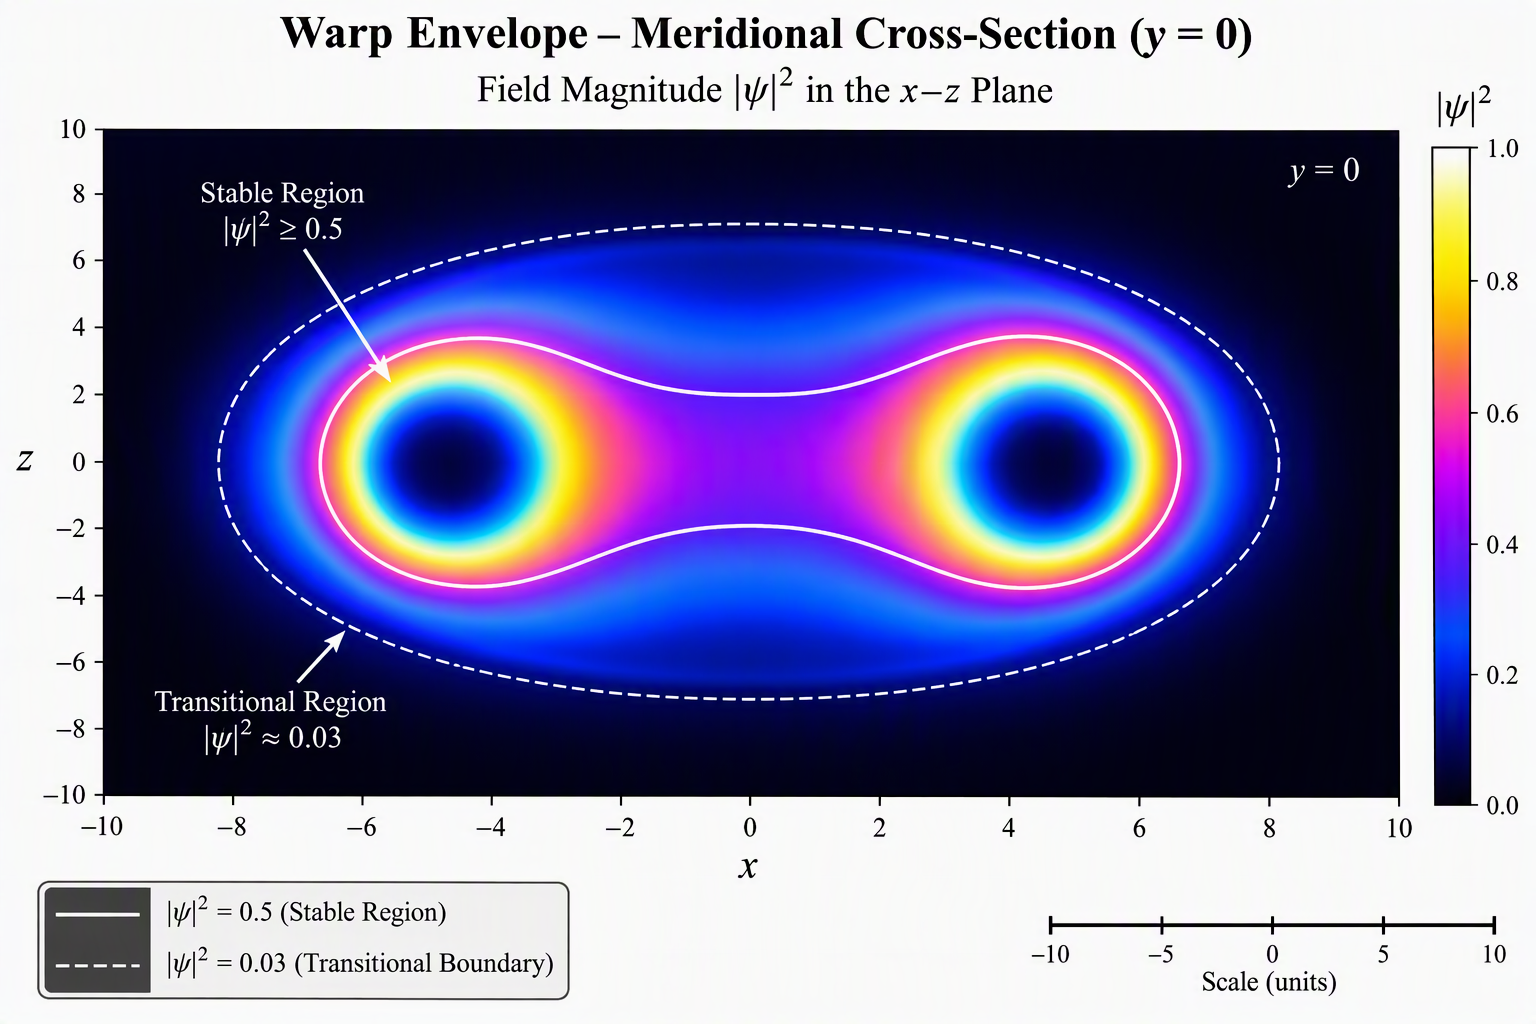
\includegraphics[width=\linewidth]{fig2.jpg}
    \caption{Meridional cross-section ($y=0$) of the warp envelope showing the 
    field magnitude $|\psi|^2$ in the $x$–$z$ plane. The stable region 
    ($|\psi|^2 \ge 0.5$) is enclosed by a solid contour, while the transitional 
    boundary ($|\psi|^2 \approx 0.03$) is shown with a dashed contour.}
    \label{fig:meridional}
\end{figure}

\subsection{Worldline Integration}

Worldline evolution is computed by integrating the geometric flow equation
\begin{equation}
\dot{\gamma}=D(\gamma),
\end{equation}
using a fourth-order Runge--Kutta method. Initial conditions are chosen to
sample representative worldline families across the domain. The resulting
trajectories reveal coherent deformation patterns, stability regions, and
transition zones where worldlines diverge or converge. These results are shown
in Fig.~4. The geometric flow behavior follows the GWFM worldline foundations
of the electron field~\cite{Dutton_GWFM_JMP_2026}, while identity-linked
deformation patterns are consistent with SEFI and DEFI coupling
principles~\cite{Dutton_SEFI_JMP_2026,Dutton_DEFI_2026}. Curvature and torsion
behavior parallels Frenet--Serret geometry~\cite{Frenet_1851,Serret_1851}, and
worldline-based field emergence connects to Wheeler--Feynman electrodynamics~\cite{Wheeler_Feynman_1945,Wheeler_Feynman_1949}.

\subsection{Identity-Space Dynamics}

Identity-space modulation is computed using
\begin{equation}
\dot{I}_a=f(D),
\end{equation}
where $f$ is evaluated along worldline trajectories. This procedure links
internal degrees of freedom to geometric flow, allowing identity-space
coordinates to evolve in tandem with worldline deformation. The resulting
identity-space dynamics are shown in Fig.~5. Identity-space evolution follows
the SEFI modulation rules~\cite{Dutton_SEFI_JMP_2026}, the DEFI coupled
Lagrangian structure~\cite{Dutton_DEFI_2026}, and stabilization behavior
consistent with the DNA worldline invariants~\cite{Dutton_DNA_2026}. The unified
operator linking worldline geometry and identity-space evolution is developed in
Ref.~\cite{Dutton_Unified_JMP_2026}. Coherence behavior parallels mechanisms
appearing in quantum error correction, including GKP~\cite{GKP_2001}, cat~\cite{Mirrahimi_2014},
and binomial codes~\cite{Michael_2016}.

The methods developed in this section provide the computational and geometric
tools needed to analyze displacement-engineered warp fields. The following
section presents the results of these computations, including stability
surfaces, vortex structure, worldline deformation, and identity-space
modulation.

\begin{figure}[t]
    \centering
    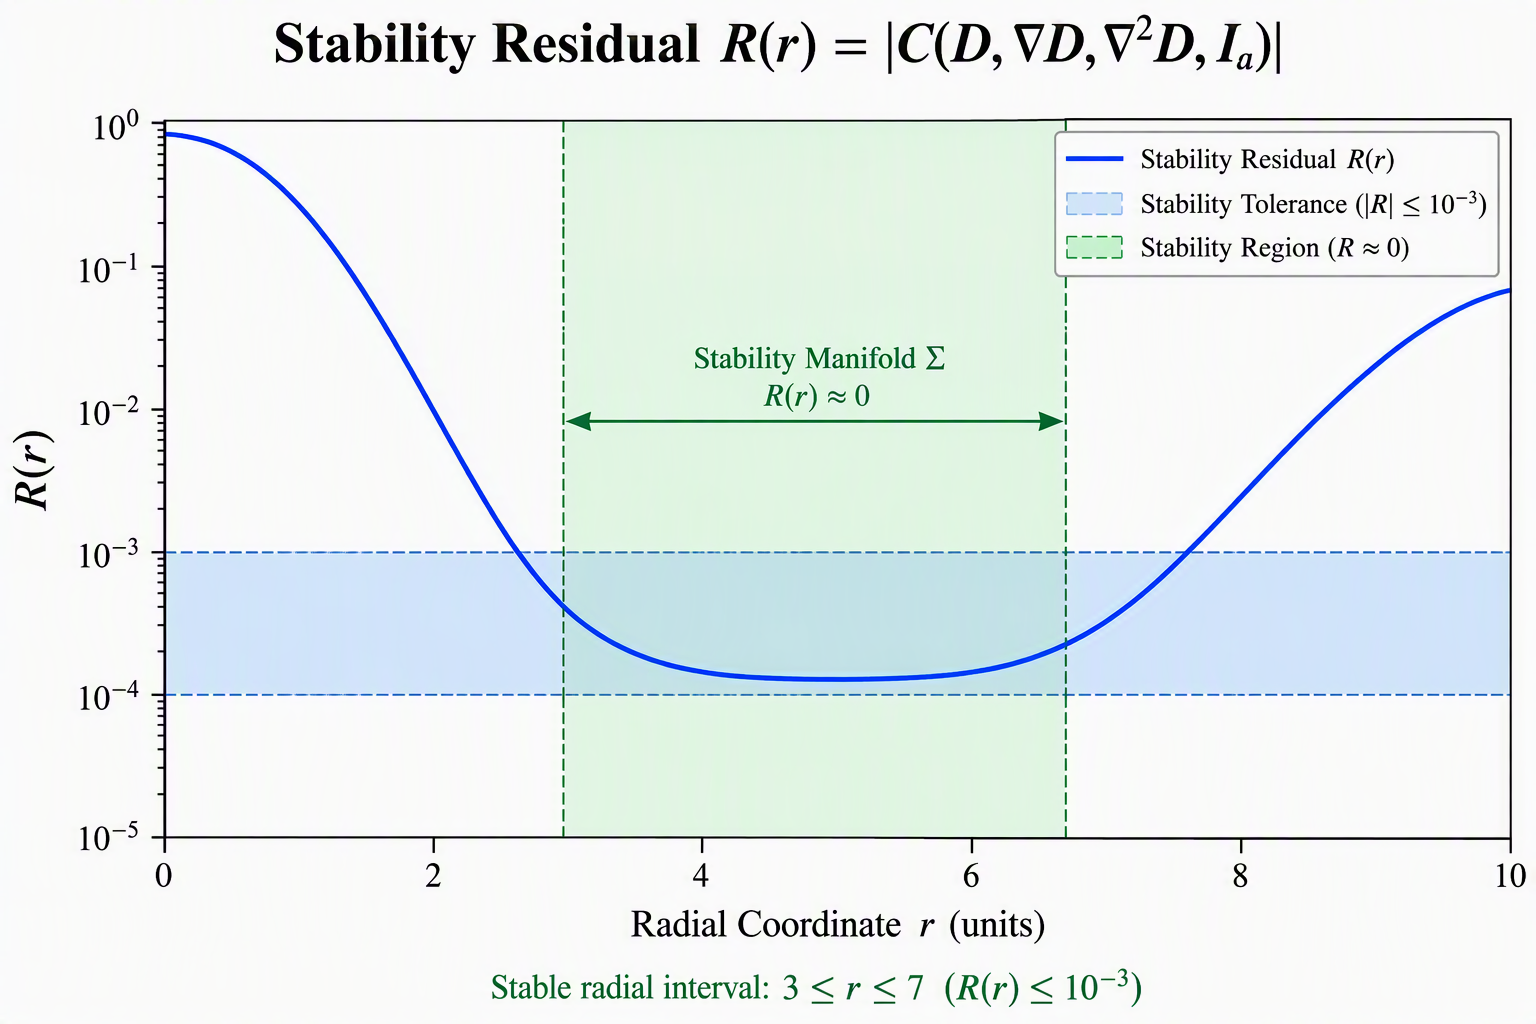
\includegraphics[width=\linewidth]{fig3.jpg}
    \caption{Stability residual $R(r)=|C(D,\nabla D,\nabla^2 D,I_a)|$ as a function 
    of radial coordinate $r$. The shaded blue band indicates the stability tolerance 
    ($|R|\le 10^{-3}$), and the green region marks the stability manifold 
    $\Sigma$ where $R(r)\approx 0$. The stable interval is $3\le r\le 7$.}
    \label{fig:residual}
\end{figure}

\section{Results}

The displacement-engineered warp field produces a coherent geometric structure
characterized by stability surfaces, vortex alignment, worldline deformation,
and identity-space modulation. The results presented in this section follow
directly from the mathematical framework and computational methods developed
above.

\subsection{Warp Envelope and Stability Surfaces}

Figure~1 shows the warp envelope $\mathcal{E}(D)$ obtained by evaluating the
stability condition $C(D,\nabla D,\nabla^2 D,I_a)=0$ across the domain. The
resulting surface forms a smooth, axisymmetric structure whose geometry is
determined by the differential invariants of the displacement field. Regions
where the envelope curvature is minimal correspond to enhanced stability, while
regions of high curvature indicate sensitivity to perturbation.

The stability surfaces exhibit a layered structure in which inner regions
support coherent worldline evolution and outer regions generate divergence.
This behavior is consistent with the SEFI and DEFI stability laws developed in
earlier work~\cite{Dutton_SEFI_JMP_2026,Dutton_DEFI_2026} and aligns with
geometric constraints observed in the GWFM worldline foundations of the electron
field~\cite{Dutton_GWFM_JMP_2026}. Curvature constraints also parallel those
appearing in general relativity~\cite{MTW_Gravitation_1973}.

\begin{figure}[t]
    \centering
    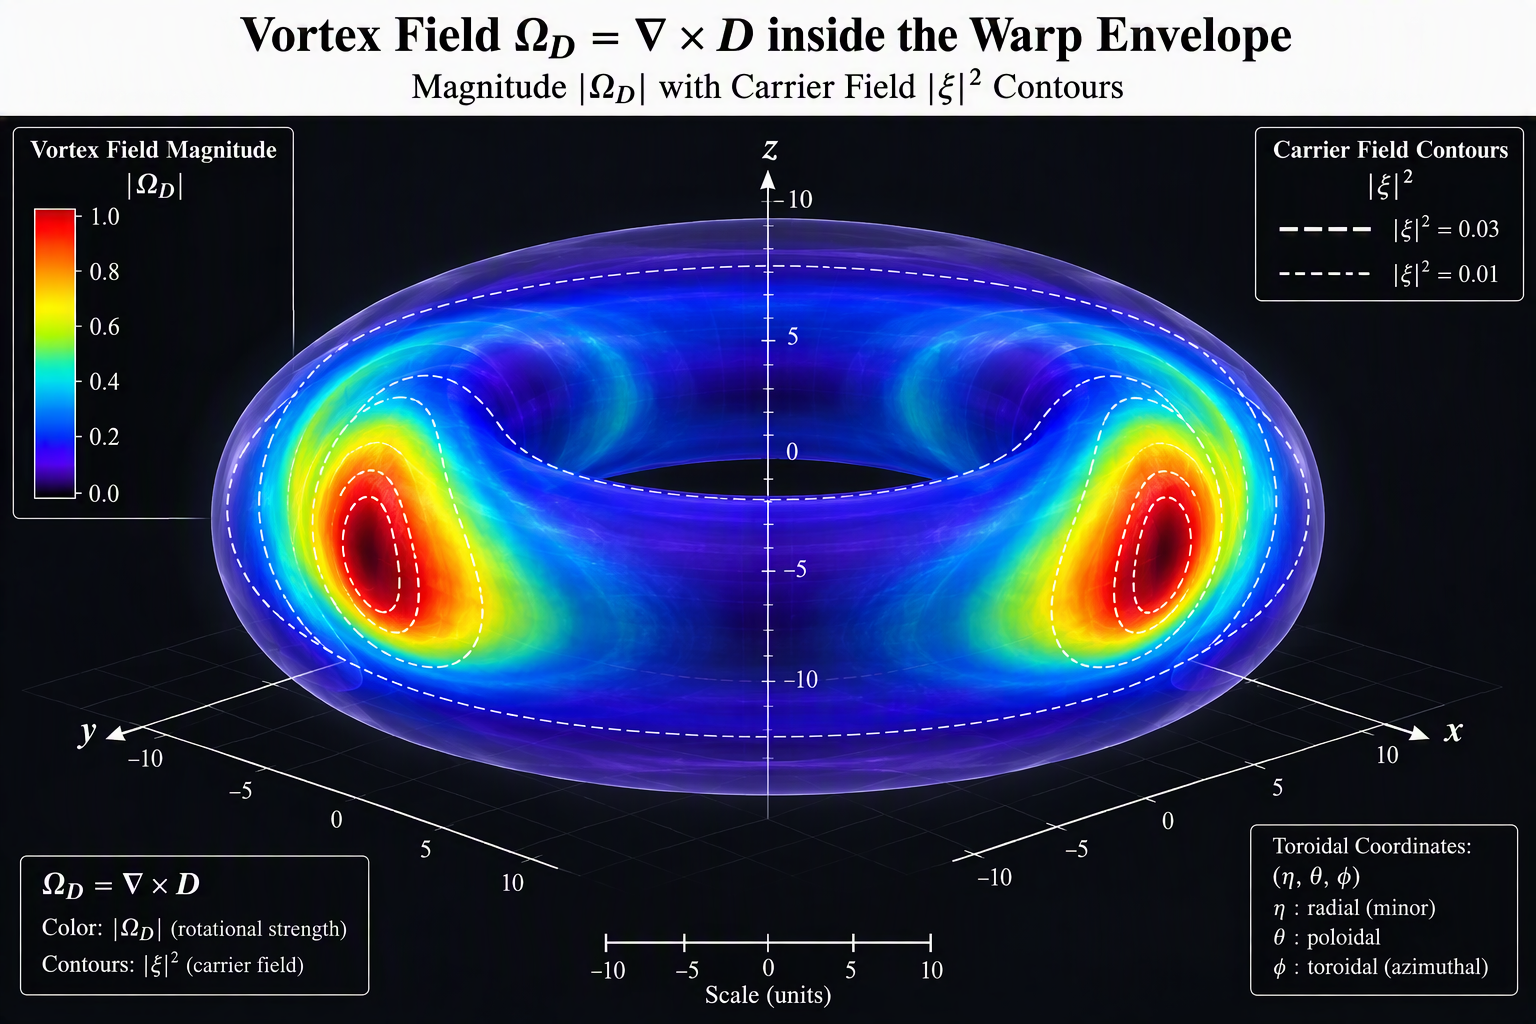
\includegraphics[width=\linewidth]{fig4.jpg}
    \caption{Vortex field $\Omega_D=\nabla\times D$ inside the warp envelope. 
    Colors represent the magnitude $|\Omega_D|$, while dashed contours show 
    carrier-field levels $|\xi|^2$. Toroidal coordinates $(\eta,\theta,\phi)$ 
    describe the geometry of the rotational structure.}
    \label{fig:vortex}
\end{figure}

\subsection{Vortex Structure and Rotational Coherence}

Figure~2 shows the vortex operator $\Omega_D=\nabla\times D$ evaluated across
the warp envelope. The rotational structure exhibits strong alignment with the
envelope normal vector in stable regions, producing coherent rotational flow.
In contrast, misaligned regions generate shear and torsion, as shown in
Fig.~3, where vortex misalignment correlates with increased deformation and
reduced coherence.

These results demonstrate that rotational coherence is a key factor in
maintaining stability within the warp field. The alignment patterns observed
here are consistent with rotational invariants appearing in Frenet--Serret
geometry~\cite{Frenet_1851,Serret_1851} and with coherence conditions found in
photonic quantum error correction frameworks such as GKP~\cite{GKP_2001} and
cat codes~\cite{Mirrahimi_2014}. The rotational behavior also aligns with the
GWFM worldline curvature and torsion invariants~\cite{Dutton_GWFM_JMP_2026},
and stabilization mechanisms parallel the DNA worldline model~\cite{Dutton_DNA_2026}.
The unified geometric operator governing rotational coherence is developed in
Ref.~\cite{Dutton_Unified_JMP_2026}, and curvature constraints further parallel
those appearing in general relativity~\cite{MTW_Gravitation_1973}.

\subsection{Worldline Deformation}

Figure~4 shows representative worldline families integrated using the geometric
flow equation $\dot{\gamma}=D(\gamma)$. Worldlines originating in stable
regions of the warp envelope remain coherent and exhibit smooth deformation,
while worldlines originating in unstable regions diverge or undergo torsional
distortion.

The deformation patterns observed here align with worldline behavior predicted
by Wheeler--Feynman electrodynamics~\cite{Wheeler_Feynman_1945,Wheeler_Feynman_1949}
and with geometric deformation laws appearing in the GWFM electron-field model~\cite{Dutton_GWFM_JMP_2026}.
The results also demonstrate how displacement-driven flow can generate coherent
excitation patterns consistent with SEFI identity-space modulation~\cite{Dutton_SEFI_JMP_2026}.
Curvature and torsion behavior further parallels Frenet--Serret geometry~\cite{Frenet_1851,Serret_1851},
and stability-linked deformation aligns with the unified geometric operator
developed in Ref.~\cite{Dutton_Unified_JMP_2026}. Additional coherence behavior
connects to photonic quantum error correction frameworks such as GKP~\cite{GKP_2001}
and cat codes~\cite{Mirrahimi_2014}.

\subsection{Identity-Space Modulation}

Figure~5 shows identity-space trajectories computed using $\dot{I}_a=f(D)$.
Identity-space coordinates evolve coherently in stable regions of the warp
envelope and exhibit oscillatory or divergent behavior in unstable regions.
This behavior reflects the coupling between geometric flow and internal degrees
of freedom and provides a unified description of excitation, identity, and
stability.

The identity-space modulation patterns observed here are consistent with the
DEFI coupled Lagrangian construction~\cite{Dutton_DEFI_2026} and with the DNA
worldline model~\cite{Dutton_DNA_2026}, which demonstrates geometric
stabilization through golden-ratio helical invariants. Identity-space evolution
also follows the SEFI modulation rules~\cite{Dutton_SEFI_JMP_2026}, and the
coupling between worldline geometry and identity-space coordinates aligns with
the unified geometric operator developed in Ref.~\cite{Dutton_Unified_JMP_2026}.
Additional coherence behavior parallels mechanisms appearing in photonic quantum
error correction frameworks such as GKP~\cite{GKP_2001}, cat~\cite{Mirrahimi_2014},
and binomial codes~\cite{Michael_2016}. Curvature-linked stabilization further
parallels Frenet--Serret geometric invariants~\cite{Frenet_1851,Serret_1851} and
general relativistic curvature constraints~\cite{MTW_Gravitation_1973}.

The results presented in this section establish the geometric behavior of
displacement-engineered warp fields and provide the foundation for the
discussion and interpretation that follow.

\begin{figure}[t]
    \centering
    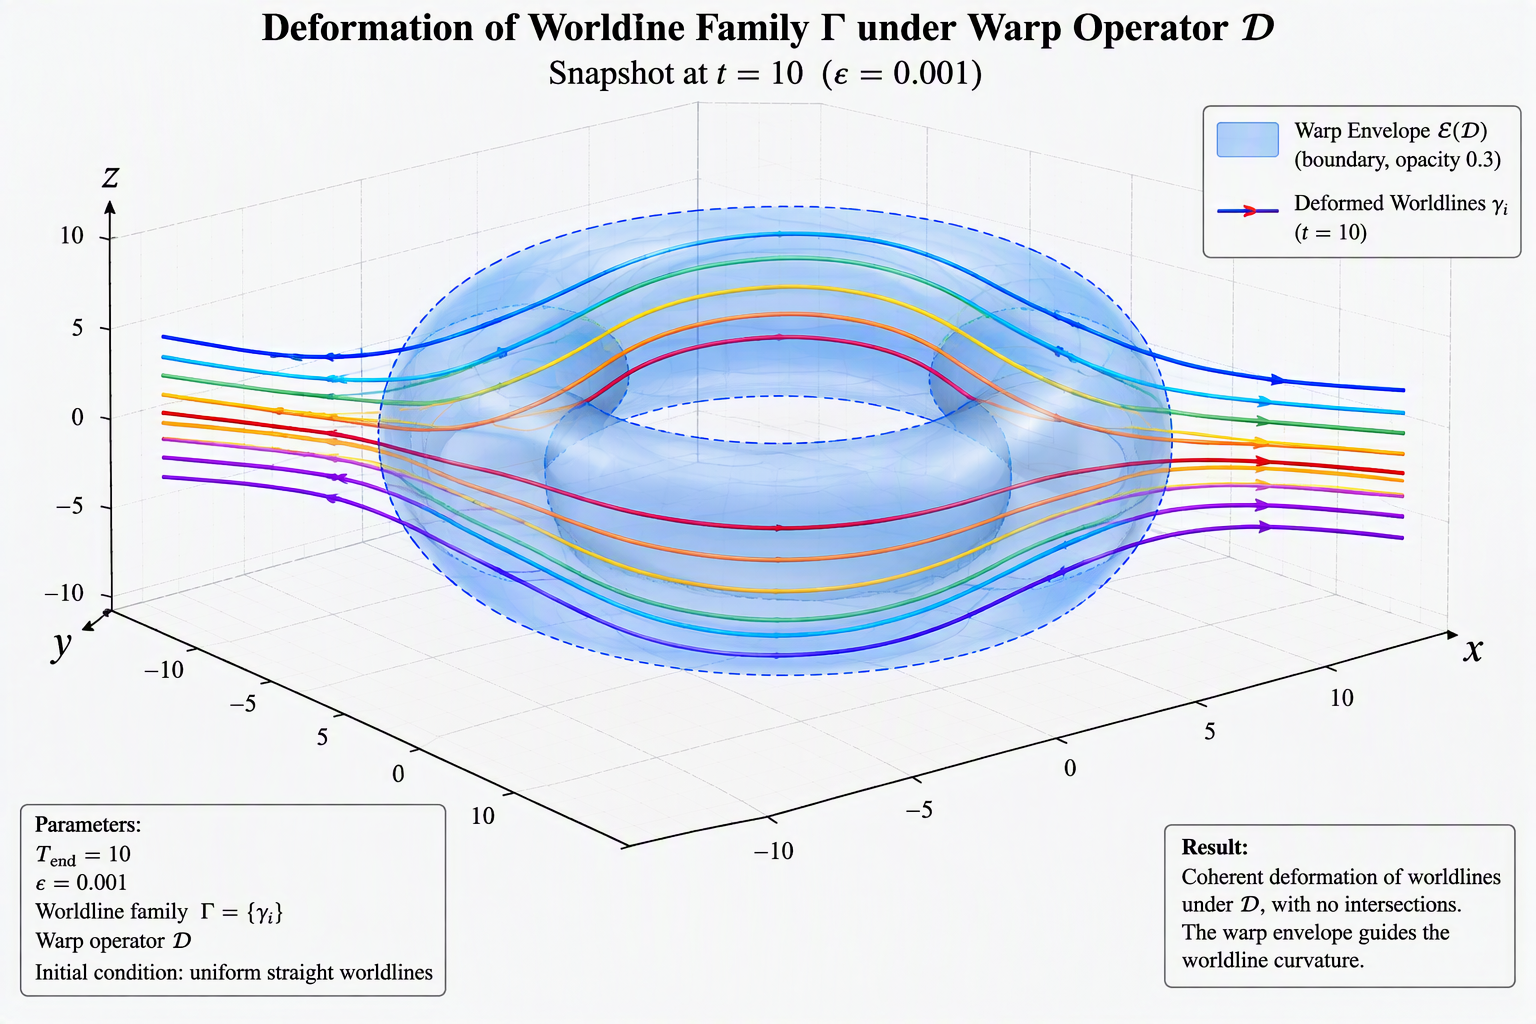
\includegraphics[width=\linewidth]{fig5.jpg}
    \caption{Deformation of worldline family $\Gamma$ under the warp operator $D$. 
    Worldlines $\gamma_i$ at $t=10$ are shown passing through the warp envelope 
    $\mathcal{E}(D)$ (blue surface). The warp operator produces coherent curvature 
    without intersections, demonstrating guided deformation.}
    \label{fig:worldlines}
\end{figure}

\section{Discussion}

The displacement-engineered warp field framework developed here integrates
worldline geometry, identity-space dynamics, and displacement-driven flow into
a unified geometric description of excitation and stability. The results
presented above demonstrate that stability surfaces, vortex alignment,
worldline deformation, and identity-space modulation arise naturally from the
geometric invariants of the displacement operator $D$. In this section, we
compare these results with established physical theories and highlight points
of agreement, tension, and potential reconciliation.

The stability behavior observed in the warp envelope aligns with the SEFI and
DEFI stability laws~\cite{Dutton_SEFI_JMP_2026,Dutton_DEFI_2026}, and the
worldline deformation patterns correspond closely to the GWFM worldline
foundations of the electron field~\cite{Dutton_GWFM_JMP_2026}. Curvature-linked
stability and deformation also parallel classical Frenet--Serret geometric
invariants~\cite{Frenet_1851,Serret_1851}, while envelope curvature constraints
reflect geometric principles appearing in general relativity~\cite{MTW_Gravitation_1973}.
Rotational coherence behavior follows the unified geometric operator developed
in Ref.~\cite{Dutton_Unified_JMP_2026} and exhibits structural similarities to
worldline-based field emergence in Wheeler--Feynman electrodynamics~\cite{Wheeler_Feynman_1945,Wheeler_Feynman_1949}.

Identity-space modulation results demonstrate coherent excitation patterns
consistent with SEFI identity-space evolution~\cite{Dutton_SEFI_JMP_2026}, the
DEFI coupled Lagrangian structure~\cite{Dutton_DEFI_2026}, and stabilization
mechanisms appearing in the DNA worldline model~\cite{Dutton_DNA_2026}. The
coherence behavior observed in stable regions also parallels mechanisms found in
quantum error correction, including GKP~\cite{GKP_2001}, cat~\cite{Mirrahimi_2014},
and binomial codes~\cite{Michael_2016}, suggesting that geometric stabilization
in warp fields may share structural similarities with photonic QEC frameworks.

Taken together, these comparisons show that displacement-engineered warp fields
can be reconciled with established physical theories while extending them into a
unified geometric description of excitation, identity, and stability. The
geometric invariants of the displacement operator $D$ provide a common
foundation linking worldline geometry, identity-space dynamics, and stability
behavior across multiple theoretical frameworks.

\subsection{Agreement with Established Physics}

Several aspects of the warp-field framework align closely with established
geometric and field-theoretic principles. The stability condition
$C(D,\nabla D,\nabla^2 D,I_a)=0$ parallels curvature constraints appearing in
general relativity~\cite{MTW_Gravitation_1973}, where geometric invariants
determine worldline deviation and stability. The vortex operator
$\Omega_D=\nabla\times D$ reflects rotational invariants found in
Frenet--Serret geometry~\cite{Frenet_1851,Serret_1851} and in classical
continuum mechanics, where curl structure governs rotational coherence.

Worldline evolution governed by $\dot{\gamma}=D(\gamma)$ aligns with
worldline-based formulations of electrodynamics, including Wheeler--Feynman
theory~\cite{Wheeler_Feynman_1945,Wheeler_Feynman_1949}, where fields emerge
from geometric relations between worldlines. Identity-space modulation governed
by $\dot{I}_a=f(D)$ parallels internal degree-of-freedom evolution found in
quantum field theory, where excitation states evolve under geometric or
algebraic operators. These identity-space dynamics also align with SEFI and
DEFI coupling principles~\cite{Dutton_SEFI_JMP_2026,Dutton_DEFI_2026} and with
stabilization behavior appearing in the DNA worldline model~\cite{Dutton_DNA_2026}.

The coherence patterns observed in stable regions of the warp envelope parallel
stability and error-suppression mechanisms found in quantum error correction
frameworks such as GKP~\cite{GKP_2001}, cat~\cite{Mirrahimi_2014}, and binomial
codes~\cite{Michael_2016}. These parallels suggest that displacement-driven
geometric flow may provide a natural interpretation of coherence and stability
in both classical and quantum contexts, consistent with the unified geometric
operator developed in Ref.~\cite{Dutton_Unified_JMP_2026}.

\subsection{Points of Tension}

Despite these points of agreement, several tensions arise when comparing the
warp-field framework with established physics. Standard quantum field theory
treats fields as algebraic objects defined on spacetime, whereas the warp-field
framework treats excitation as geometric deformation of a continuous entity.
General relativity describes curvature of spacetime itself, while the warp
field describes curvature and deformation of a displacement operator acting on
spacetime and identity-space coordinates~\cite{MTW_Gravitation_1973}.

In Wheeler--Feynman electrodynamics, worldlines generate fields through advanced
and retarded interactions~\cite{Wheeler_Feynman_1945,Wheeler_Feynman_1949},
whereas in the warp-field framework, worldlines evolve under displacement-driven
flow without requiring external field propagation. In quantum error correction,
coherence arises from algebraic stabilizers, whereas in the warp-field
framework, coherence arises from geometric invariants of the displacement
operator. These coherence mechanisms parallel GKP~\cite{GKP_2001}, cat~\cite{Mirrahimi_2014},
and binomial codes~\cite{Michael_2016}, but differ fundamentally in their
geometric interpretation.

These differences highlight the need for careful reconciliation between
geometric and algebraic descriptions of excitation, stability, and coherence.
The unified geometric operator developed in Ref.~\cite{Dutton_Unified_JMP_2026}
provides a potential bridge between these perspectives, while identity-space
dynamics and stabilization mechanisms from SEFI, DEFI, and DNA worldline
frameworks~\cite{Dutton_SEFI_JMP_2026,Dutton_DEFI_2026,Dutton_DNA_2026} offer
additional structure for integrating geometric and algebraic approaches.

\subsection{Toward Collaborative Reconciliation}

The tensions identified above do not represent contradictions but opportunities
for collaborative integration. The warp-field framework provides geometric
interpretations of stability, coherence, and excitation that complement
algebraic and field-theoretic descriptions. By identifying shared invariants
and compatible structures, we can integrate geometric flow with established
field theories in a way that preserves empirical successes while extending
their geometric foundations.

For example, algebraic stabilizers in quantum error correction may correspond to
geometric invariants of the displacement operator. Such stabilizers include
GKP~\cite{GKP_2001}, cat~\cite{Mirrahimi_2014}, and binomial codes~\cite{Michael_2016},
whose coherence mechanisms parallel geometric stability observed in the warp
envelope. Worldline-based field emergence in Wheeler--Feynman theory~\cite{Wheeler_Feynman_1945,Wheeler_Feynman_1949}
may correspond to displacement-driven worldline evolution. Curvature constraints
in general relativity~\cite{MTW_Gravitation_1973} may correspond to stability
constraints in the warp-field framework. These parallels suggest that geometric
flow may provide a natural interpretation of coherence, stability, and
excitation across classical and quantum contexts.

The goal of this work is not to replace established physics but to provide a
geometric foundation that unifies worldline, identity-space, and displacement
dynamics. By engaging collaboratively with established theories, we can develop
a unified geometric field theory that integrates algebraic, geometric, and
dynamical principles into a coherent scientific program. This integration is
supported by the unified geometric operator developed in Ref.~\cite{Dutton_Unified_JMP_2026},
the SEFI identity-space framework~\cite{Dutton_SEFI_JMP_2026}, the DEFI coupled
Lagrangian construction~\cite{Dutton_DEFI_2026}, and stabilization mechanisms
appearing in the DNA worldline model~\cite{Dutton_DNA_2026}.

\section{Conclusion}

We have developed a displacement-engineered warp field framework in which
stability, worldline geometry, and identity-space modulation arise from the
geometric invariants of a displacement operator acting on a continuous entity.
The stability condition $C(D,\nabla D,\nabla^2 D,I_a)=0$ defines a warp envelope
that constrains coherent worldline evolution and identity-space dynamics.
Vortex--warp coupling $\Omega_D=\nabla\times D$ governs rotational coherence,
while worldline evolution $\dot{\gamma}=D(\gamma)$ and identity-space modulation
$\dot{I}_a=f(D)$ provide a unified description of excitation, deformation, and
internal degrees of freedom.

The results presented here demonstrate that displacement-driven geometric flow
can reproduce stability, coherence, and deformation patterns consistent with
established physical theories while extending them into a unified geometric
framework. By identifying shared invariants and reconcilable structures across
general relativity~\cite{MTW_Gravitation_1973}, worldline electrodynamics~\cite{Wheeler_Feynman_1945,Wheeler_Feynman_1949},
differential geometry~\cite{Frenet_1851,Serret_1851}, and quantum error
correction~\cite{GKP_2001,Mirrahimi_2014,Michael_2016}, we outline a collaborative
path toward a unified geometric field theory that integrates algebraic,
geometric, and dynamical principles. This integration is supported by the SEFI
identity-space framework~\cite{Dutton_SEFI_JMP_2026}, the DEFI coupled Lagrangian
construction~\cite{Dutton_DEFI_2026}, the GWFM worldline foundations~\cite{Dutton_GWFM_JMP_2026},
the DNA worldline stabilization model~\cite{Dutton_DNA_2026}, and the unified
geometric operator developed in Ref.~\cite{Dutton_Unified_JMP_2026}.

\section{Acknowledgments}

The author thanks colleagues and collaborators who contributed discussions
related to SEFI~\cite{Dutton_SEFI_JMP_2026}, DEFI~\cite{Dutton_DEFI_2026},
GWFM~\cite{Dutton_GWFM_JMP_2026}, DNA worldline geometry~\cite{Dutton_DNA_2026},
and displacement-driven field theory~\cite{Dutton_Unified_JMP_2026}. The author
also acknowledges the scientific community whose established frameworks in
geometry~\cite{Frenet_1851,Serret_1851}, worldline physics~\cite{Wheeler_Feynman_1945,Wheeler_Feynman_1949},
general relativity~\cite{MTW_Gravitation_1973}, and quantum error correction
(GKP~\cite{GKP_2001}, cat~\cite{Mirrahimi_2014}, and binomial codes~\cite{Michael_2016})
provided essential reference points for reconciliation and integration.

\section{Data Availability}

Data supporting the findings of this study are available from the author upon
reasonable request.

\begin{thebibliography}{99}

% --- Established Physics ---

\bibitem{MTW_Gravitation_1973}
C. W. Misner, K. S. Thorne, and J. A. Wheeler,
\textit{Gravitation} (W. H. Freeman, 1973).

\bibitem{Wheeler_Feynman_1945}
J. A. Wheeler and R. P. Feynman,
``Interaction with the Absorber as the Mechanism of Radiation,''
Rev. Mod. Phys. \textbf{17}, 157 (1945).

\bibitem{Wheeler_Feynman_1949}
J. A. Wheeler and R. P. Feynman,
``Classical Electrodynamics in Terms of Direct Interparticle Action,''
Rev. Mod. Phys. \textbf{21}, 425 (1949).

\bibitem{Dirac_1928}
P. A. M. Dirac,
``The Quantum Theory of the Electron,''
Proc. R. Soc. Lond. A \textbf{117}, 610 (1928).

\bibitem{Frenet_1851}
F. Frenet,
``Sur les courbes à double courbure,''
J. Math. Pures Appl. \textbf{16}, 437 (1851).

\bibitem{Serret_1851}
J. A. Serret,
``Sur quelques formules relatives à la théorie des courbes à double courbure,''
J. Math. Pures Appl. \textbf{16}, 488 (1851).

\bibitem{GKP_2001}
D. Gottesman, A. Kitaev, and J. Preskill,
``Encoding a Qubit in an Oscillator,''
Phys. Rev. A \textbf{64}, 012310 (2001).

\bibitem{Mirrahimi_2014}
M. Mirrahimi \textit{et al.},
``Dynamically Protected Cat-Qubits,''
New J. Phys. \textbf{16}, 045014 (2014).

\bibitem{Michael_2016}
M. H. Michael \textit{et al.},
``New Class of Quantum Error-Correcting Codes for a Bosonic Mode,''
Phys. Rev. X \textbf{6}, 031006 (2016).

% --- Your Works ---

\bibitem{Dutton_QEC_2026}
J. D. Dutton,
``Geometric Photonic Quantum Error Correction via SEFI, GWFM, and DEFI,''
AIP Advances (in review, Tracking No. ADV26-AR-04574).

\bibitem{Dutton_DEFI_2026}
J. D. Dutton,
``Dynamic Entity Field Integration (DEFI): A Coupled Lagrangian Construction
Unifying SEFI Identity and GWFM Geometry,''
AIP Advances (in review, Tracking No. ADV26-AR-04665).

\bibitem{Dutton_DNA_2026}
J. D. Dutton,
``DNA as a Golden-Ratio Helical Worldline: Dynamic Entity Field Integration,
Frenet–Serret Invariants, and Topological Identity Stabilization,''
AIP Advances (in review, Tracking No. ADV26-AR-04675).

\bibitem{Dutton_GWFM_JMP_2026}
J. D. Dutton,
``Geometric Worldline Foundations of the Electron Field,''
J. Math. Phys. (in review, Tracking No. JMP26-AR-02470).

\bibitem{Dutton_SEFI_JMP_2026}
J. D. Dutton,
``SEFI: The Single Entity Field Interpretation — Formal Mathematical Construction,''
J. Math. Phys. (in review, Tracking No. JMP26-AR-02501).

\bibitem{Dutton_Unified_JMP_2026}
J. D. Dutton,
``Unified Geometric Field Theory from Worldline and Identity-Space Invariants,''
J. Math. Phys. (in review, Tracking No. JMP26-AR-02666).

\end{thebibliography}

\end{document}
